\chapter{Sources of Intelligence}

\section{Herramientas de Ciberconciencia Situacional}
Las herramientas de ciberconciencia situacional (CSA) son necesarias porque los sistemas de monitorización de ciberseguridad y las herramientas de ciberinteligencia generan enormes cantidades de información que resultaría imposible analizar manualmente. Este análisis manual sería laborioso y propenso a errores. Además, un problema crítico es que los analistas pueden "ahogarse en un mar de detalles" y perder la visión global de la situación.

\subsection{Objetivos principales}
Las herramientas de CSA deben mejorar el rendimiento, la cognición y la comprensión tanto para analistas como para responsables de toma de decisiones. Específicamente, ayudan a responder preguntas fundamentales como:
\begin{itemize}
   \item ¿Hay algún ataque en curso? Si es así, ¿dónde está el atacante? ¿Cómo evoluciona la situación?
   \item ¿Cómo está afectando el ataque a la empresa o misión? ¿Cómo podemos evaluar el daño?
   \item ¿Cómo se espera que se comporten los atacantes? ¿Cuáles son sus estrategias?
   \item ¿Podemos predecir futuros plausibles de la situación actual?
   \item ¿Cómo creó el atacante la situación actual? ¿Qué intentaba conseguir?
\end{itemize}

\subsection{Diferenciación con otras herramientas}
Estas preguntas no pueden ser respondidas por otras herramientas de ciberseguridad o ciberinteligencia convencionales:
\begin{itemize}
   \item Un IDS no proporciona percepción situacional, pues ésta va más allá de la simple detección de eventos
   \item Un SIEM puede correlacionar eventos, pero no proporciona un Common Operational Picture (COP) como paso previo para generar sensemaking
   \item Un sistema de detección de vulnerabilidades (VDS) produce una vista estática de vulnerabilidades, pero no la correlaciona con información de incidentes en tiempo real
   \item Las diferentes herramientas de inteligencia (HUMINT, OSINT, SIGINT, TECHINT) generan su propio tipo de conocimiento que debe ser correlacionado
\end{itemize}

\subsection{Capacidades clave}
Según la OTAN (Multinational Cyber Defence Capability Development), las herramientas de CSA deben incluir capacidades como:
\begin{itemize}
   \item Visualizar listas de riesgos actuales, ordenados por impacto y con localización geográfica
   \item Generación de informes con diferentes niveles de detalle (drill down/roll up)
   \item Vistas jerárquicas personalizadas
   \item Seguridad de datos basada en unidad y localización
   \item Visualización de dependencias entre activos
   \item Agregación de incidentes por región geográfica o por red, con vistas enlazadas
   \item Generación y selección de cursos de acción posibles
   \item Fusión de datos de múltiples fuentes
   \item Gestión de vistas y paneles de control
   \item Capacidades avanzadas de visualización y simulación
\end{itemize}

\subsection{Requisitos operacionales}
El proyecto PANOPTESEC estableció requisitos fundamentales para estas herramientas, que incluyen:
\begin{itemize}
   \item \textbf{Para fuentes y recolección de datos:} Interfaces estándar y no estándar para la recolección de datos de múltiples fuentes, capacidad de almacenar datos en bruto, recolección de información de configuración de sistemas, información sobre dispositivos, sistemas operativos, aplicaciones, topología de red, etc.
   
   \item \textbf{Para correlación de datos:} Motor de correlación de información que traduzca datos de múltiples fuentes a una representación común, identificación de elementos comunes, resolución de conflictos entre elementos informativos, creación de una vista unificada del sistema monitorizado y un modelo de impacto en la misión.
   
   \item \textbf{Para visualización:} Sistema que muestre la conciencia situacional de ciberdefensa en tiempo real, representando niveles de riesgo en estado estable y dinámico, impacto anticipado en la misión, detalles sobre sistemas críticos, información sobre topología de red, vulnerabilidades, rutas de ataque, y eventos de seguridad en tiempo real, así como acciones de mitigación propuestas.
\end{itemize}

\section{Connection of Cyber Sensors}
If we are to connect two systems to exchange data about assets (the same applies
to threats, vulnerabilities, etc.) we have to agree on:
\begin{itemize}
    \item What is an asset and what features and properties does it have
    \begin{itemize}
      \item From a format perspective
      \item Syntactically
      \item Semantically
   \end{itemize}
    \item How to exchange that data in an automatic and standard way between any given systems
\end{itemize}

This leads to the definition of standards for elements characterization and exchange, such as:
\begin{itemize}
   \item SCAP - Security Content Automation Protocol
   \item Assets
   \begin{itemize}
      \item ARF - Asset Reporting Format
      \item AI - Asset Identification
      \item CPE - Common Platform Enumeration 
   \end{itemize}
   
   \item Vulnerabilities
   \begin{itemize}
      \item CVE - Common Vulnerabilities Enumeration
      \item CVSS - Common Vulnerability Scoring System
      \item CWE - Common Weakness Enumeration
      \item OSVDB - Open Source Vulnerability Database
      \item CVRF - Common Vulnerability Reporting Framework
   \end{itemize}
   \item Threats
   \begin{itemize}
   	\item STIX - Structured Threat Information eXpression
	   \item TAXII  - Trusted Automated eXchange of Indicator Information
	   \item MAEC - Malware Attribute Enumeration and Characterization
	   \item CAPEC - Common Attack Pattern Enumeration and Classification
	   \item CybOX - Cyber Observable eXpression
   \end{itemize}
   \item etc\dots
\end{itemize}

Tipicamente, la comunicación entre sensores y sistemas se hace con XML (sorprendentemente predominante) o JSON, pero hay también enfoques basados en REST o proprietary APIs. El workflow planea de obtener informaciones de varios tipos de distintas fuentes, integrar las informaciones, correrlarlas, y finalmente generar ciberconciencia situacional.
\labelitemize{Enfoques}{
   \begin{enumerate}
      \item Comunicación directa entre sistemas a través de uno exchange standard, como ARF o STIX
      \item Federation/Middleware: un sistema centralizado que recibe datos de los sensores y los distribuye a otros sistemas
      \item Subscription: hay un cloud de servidores para enviar datos a través de mecanismos propios. 
      \note{Por la mayor parte, estos sistemas son de pago y no open source.}
      \item Common Collaborative Repository: Se uploadean datos a un repositorio comúm confiable y autorizado, cómo algunos SIEMs, CVE, \dots
   \end{enumerate}
}

\newpage
\section{SIEM}
\begin{paracol}{2}
   SIEM stands for Security Information and Event Management. It is a system that
   collects and aggregates log data from many different sources, normalizes the
   data, correlates it, and then alerts based on rules and heuristics.
   Tipicamente es un elemento centralizado que gestiona una subred, o parte de una.
   
   \note{\begin{itemize}
      \item Splunk
      \item QRadar
      \item OSSIM
      \item AlienVault USM (old)
   \end{itemize}}
   \switchcolumn

   \begin{figure}[htbp]
      \centering
      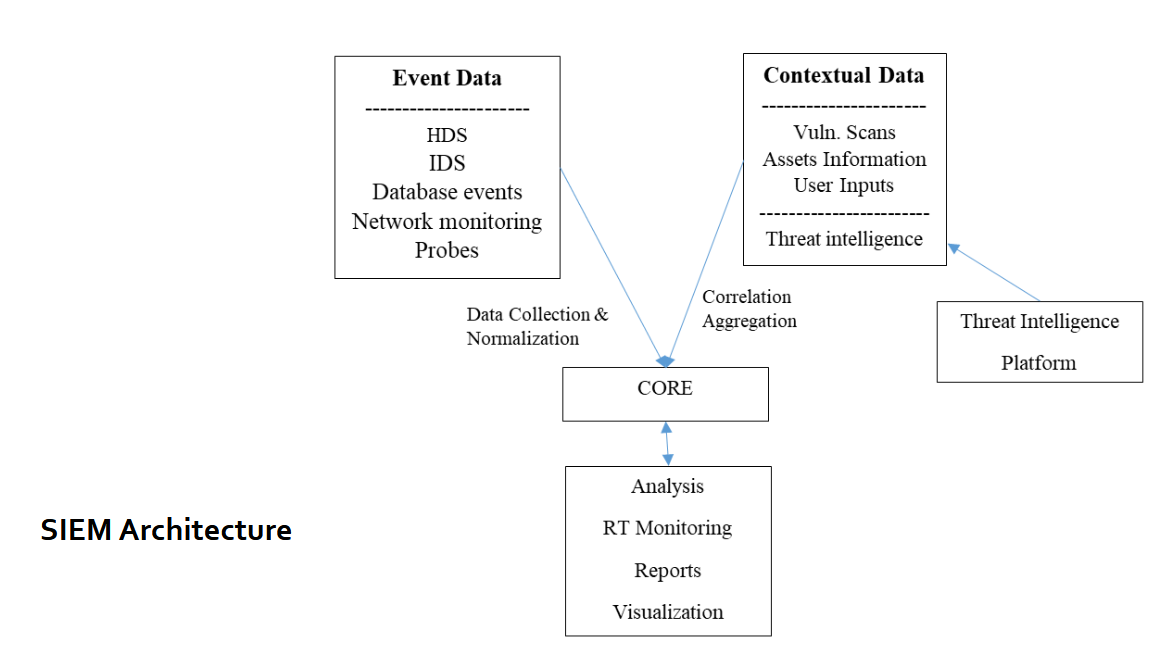
\includegraphics{images/04/SIEM.png}
      \caption{SIEM Architecture}
      \label{fig:04/SIEM}
   \end{figure}

\end{paracol}

\section{Incident Response Systems}

Based on existing ticketing systems, they allow insertion, storing and management of incidents on a central
point, aiming at providing response coordination and proper management among interested parties.

They are designed to be integrated with TIPs (Threat Management Platform?) and SIEMs, and to help \textit{Computer Incident Response Team} (\textsc{CIRT}) members carry out
incident handling properly, providing workflow management and logs of what happened, when and how about the incident and the response.